\subsection{TCP Vegas}

\subsubsection{Congestion avoidance}

Reaction to congestion episode, not to packets loss
Modifications:
\begin{itemize}
  \item Modified Congestion Avoidance
  \item Aggressive Retransmission
  \item Aggressive Window Adaptation
  \item Modified SS phase
\end{itemize}

Some definitions:
\begin{itemize}
  \item \textbf{Throughput}: speed of transmission
  \item \textbf{Goodput}: speed of reception
\end{itemize}

\noindent Comparing expected throughput\dots
\begin{equation*}
Expected\ throughput = \frac{window\ size}{RTT}
\end{equation*}
\dots and actual throughput:
\begin{equation*}
Actual\ throughput: \frac{actual\ transmitted\ amount}{RTT}
\end{equation*}

\noindent Monitor transmission rate:
\begin{itemize}
\item If $expected - \alpha < actual < expected$: Queues decreasing
  $\rightarrow$ increase rate
\item If $expected - \alpha < actual < expected - \beta$: Don’t do anything
\item If $actual < expected - \beta$: Queues increasing $\rightarrow$ decrease
  rate before packet drop (maybe there is a congestion in network or maybe the
  connection is shared among other services) 
\end{itemize}

Thresholds of $\alpha (= \frac{1 pkts}{RTT})$ and
$\beta (= \frac{3 pkts}{RTT})$ correspond to how many packets Vegas is willing
to have in queues.
\begin{figure}[t]
  \centering
  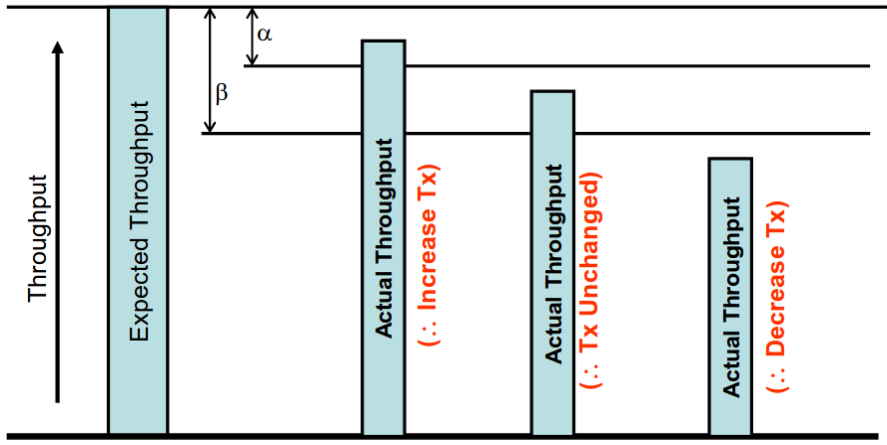
\includegraphics[scale=0.35]{CAVegas}
  \caption{Vegas - Modified Congestion Avoidance}
  \label{fig:tcpVegas:mca}
\end{figure}




